%====================================================
%	CHAPTER 4 - Control
%====================================================
\chapter{Controller Development}
\label{ch:control}
%====================================================
\section{Control Loop}
%====================================================
The control problem for this dissertation is, as outlined in Chater:\ref{ch:intro}; to achieve dynamic (\emph{attitude}) set point tracking on a quadrotor by solving the problem of its inherent underactuation. For the purposes of the subsequent controller development, the plant is described in the following non-linear state space form:
\begin{subequations}
\begin{equation}
\dot{\mathbf{x}}=f(\mathbf{x},t)+g(\mathbf{x},\vec{\nu},t)
\end{equation}
\vspace{-15pt}
\begin{equation}
y = c(\mathbf{x},t)+d(\mathbf{x},\vec{\nu},t)
\end{equation}
\end{subequations}
Where the plant dynamics are governed by $f(\mathbf{x},t)$ and the plant's input response by $g(\mathbf{x},\vec{\nu},t)$, for a given input $\vec{\nu}$. The latter is not necessarily a function based relationship and could take a multiplicative form; $g(\mathbf{x},t)\vec{\nu}$. The objective for setpoint tracking is for the output to track the state $y = \mathbf{x}$. As such, the control problem is to design a stabilizing control law for an error state $\mathbf{x}_e$\footnote{Ignoring how error states are formulated for the time being\ldots}:
\\
\vspace{-5pt}
\begin{equation}
\vec{\nu}_d=h(\mathbf{x}_e,t)
\end{equation}
Such that the control plant is globally asymptotically stable or that $\lim_{t\rightarrow\infty}\mathbf{x}_e=0$. It is possible to combine attitude and position states into a common trajectory state such that:
\\
\vspace{-5pt}
\begin{equation}
\mathbf{x}=\begin{bmatrix}
\vec{\mathcal{E}}\\
Q_b
\end{bmatrix}
\end{equation}
The body's trajectory is then fully described by $\mathbf{x}(t)$. Separate control laws are developed for attitude and position tracking and hence those states aren't combined. However for the purposes of discussing the control plant, a single major loop is considered. The designed control input, $\vec{\nu}_d$, is then implemented by actuator suite $u\in\mathbb{U}$ through its effectiveness function:
\\
\vspace{-5pt}
\begin{equation}
\nu_c=B(\mathbf{x},u,t)
\end{equation}
The exact relationship of the virtual control input and commanded input, $\nu_c\rightarrow\nu_d$, is governed by the allocation algorithm. That allocation function, $B^\dagger$, can be \emph{approximately} referred to as the effectiveness inverse. The actuator positions are then solved subject to some constraint as:
\begin{equation}
u=B^{\dagger}(\mathbf{x},\nu_d,t)
\end{equation}
The control allocation requirements and schemes are expanded upon subsequently in Section:\ref{sec:control.allocation}. Multiple attitude controllers are presented whose stability is proved with Lyapunov$^\dagger$ stability theorem. Each controller is compared in the context of an over actuated quadrotor plant. Similarly a series of allocation schemes are compared too. Those comparisons, their details and how controller efficacy is evaluated are all presented next in Chapter:\ref{ch:simulation}. 
\newpage
The generalized over-actuated control loop is split into a series of blocks, illustrated in Fig:\ref{fig:control-loop}. From the error state of the generated trajectory, $\mathbf{x}_e$, the control law designs a virtual control input, $\vec{\nu}_d$, which is cast as the argument to the allocation block. From the allocation law, $B^{\dagger}$, physical actuator positions are obtained; $u\in\mathbb{U}$. Those actuator positions effect a virtual plant input, $\vec{\nu}_c$, which is an input to further the state function. Not shown, but implied in Fig:\ref{fig:control-loop}, is the state derivative feedback of $\dot{\mathbf{x}}$ to the plant transfer function. Finally the output tracking state is estimated with some filtration paradigm, $\hat{\mathbf{x}}=A(\mathbf{x},t)$, and fed back to the error state.
\begin{figure}[htbp]
\centering
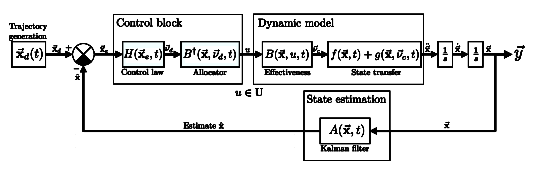
\includegraphics[width=\textwidth]{figs/control-loop}
\caption{Generalized control loop with allocation}
\label{fig:control-loop}
\end{figure}
%====================================================
\section{Control Plant Inputs}
\label{sec:control.inputs}
%====================================================
Thus far control plant inputs for the set of differential state equations, from Eq:\ref{eq:quaternion-states}, have mostly been described with net forces and torques; $\mu\vec{F}$ \& $\mu\vec{\tau}$. The relationship between propeller rotational speeds \& servo positions and the resultant thrust vector directions are calculated as in Eq:\ref{eq:quaternion-inputs}.
\begin{subequations}\label{eq:control-input}
\begin{equation}
\mu\vec{F}(u)=\sum Q_{M_i}^*(\lambda_i,\alpha_i)\otimes T(\Omega_i)\otimes Q_{M_i}(\lambda_i,\alpha_i)~~~~\in\mathcal{F}^b
\end{equation}
\vspace{-10pt}
\begin{equation}
\mu\vec{\tau}(u)=\sum \vec{l}\times\big(Q_{M_i}^*(\lambda_i,\alpha_i)\otimes T(\Omega_i)\otimes Q_{M_i}(\lambda_i,\alpha_i)\big)~~~~\in\mathcal{F}^b
\end{equation}
\end{subequations}
To accommodate comparison of each controller and allocation scheme, the error state control law(s) design net plant inputs $\mu\vec{F}$ and $\mu\vec{\tau}$. The allocation rule then takes those net inputs as an arguments to find actuator positions to effect those net inputs. As such each control law can be tested against various allocation rules and \emph{vise versa}. However typical allocation algorithms, like pseudo-inversion, require a multiplicative relationship between plant and control inputs\ldots 
\par
The actuator effectiveness functions in Eq:\ref{eq:control-input} aren't readily reducible to a single multiplicative relationship. Thusly the effectiveness function needs an extra layer of abstraction to incorporate a multiplicative relationship. Rather than calculating actuator positions directly from $\vec{\nu}_d$, a set of four 3-dimensional thrust vectors, $\vec{T}_{1\rightarrow 4}$, for each motor module are calculated first.
\begin{equation}
\vec{\nu}_d=\begin{bmatrix}
\mu\vec{F}\\
\mu\vec{\tau}
\end{bmatrix}
= 
\begin{bmatrix}
1 & 1 & 1 & 1\\
\vec{l}_\times & \vec{l}_\times & \vec{l}_\times & \vec{l}_\times
\end{bmatrix}
\begin{bmatrix}
\vec{T}_1\\
\vec{T}_2\\
\vec{T}_3\\
\vec{T}_4
\end{bmatrix}
\end{equation}
Where $\vec{l}_\times$ is the cross product vector of the torque arm. Individual actuator positions for each module, $[\Omega,~\lambda,~\alpha]^T$, can be calculated from those thrust vectors $\vec{T}_i$ for $i\in[1:4]$ with some trigonometry, ensuring that they only adhere to Eq:\ref{eq:control-input}. That trigonometric inversion\footnote{Inverting either rotation matrix operations or quaternions} can be described as the function $R^\dagger$:
\begin{equation}
[\Omega_i,~\lambda_i,~\alpha_i]^T=R^\dagger(\mathbf{x},\vec{F}_i,t)~~~~i\in[1:4]
\end{equation}
\par
To summarize then; each allocation rule controls designs net thrust vectors for each of the four modules in the following form:
\begin{equation}
B^{\dagger}(\mathbf{x},\vec{\nu}_d,t)=\big[ T_{1x},~T_{1y},~T_{1z},~\ldots~T_{4x},~T_{4y},~T_{4z}\big]^T
\end{equation}
The control block in the loop (Fig:\ref{fig:control-loop}) is then modified to incorporate the extra abstraction level, shown in Fig:\ref{fig:control-block}. The output from that control block is still the same actuator matrix $u\in\mathbb{U}$. The block merely accommodates for comparison of various allocation rules without compromising the entire loop's structure.
\begin{figure}[htbp]
\centering
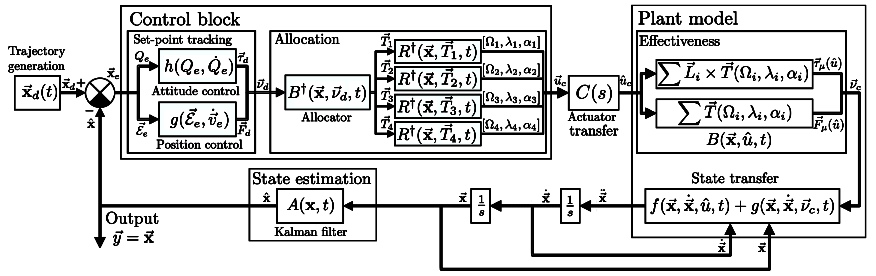
\includegraphics[width=0.7\textwidth]{figs/control-block}
\caption{Abstracted control block}
\label{fig:control-block}
\end{figure}
\par
\emph{\color{Gray} Al allocation algorithms proposed follow the structure described in Fig:\ref{fig:control-block}. One allocation algorithm does, however, circumvent the virtual abstraction level of thrust vector's for each module to directly calculate actuator positions.}
\par
Each control law is co-dependent with an accompanying allocation algorithm. Traditional control loops (under-actuated or well matched) typically have a unity allocation algorithm and as such require no consideration so they're mostly disregarded. Separate control laws for attitude ad position control are presented next in Section:\ref{sec:control.attitude} and \ref{sec:control.position} respectively. Thereafter a series of allocation rules are proposed in Section:\ref{sec:control.allocation}. Although presented independently, the controller and allocation laws are mutually inclusive. The stability of each control law is proven objectively but actual controller tuning and optimization takes place only later in Section:\ref{sec:simulation.tuning}.
\par
%====================================================
\subsection*{Model Dependent \& Independent Controllers}
%====================================================
Two classes of controllers are presented, attitude and position control laws. The former being the primary focus of this research project and containing a more verbose control treatment. Both control categories consider MIMO state vector loops for $\mathcal{E}$ \& $Q_b$. The allocation algorithm combines virtual control inputs $\vec{\mu}_d=[\mu\vec{F}~\mu\vec{\tau}]^T$ generated from the two control categories.
\par
The control dependency on the system plant is as a consequence of the prominent actuator response dynamics, as derived previously in Section:\ref{subsec:dynamics.nonlinearities.gyrotorques} from Chapter:\ref{ch:dynamics}. Whilst not a prerequisite for stability, plant dependent compensation certainly improves controller performances. Independent and dependent cases are only presented in one type of controller; the basic case PD controller in Section:\ref{subsec:control.attitude.controllers}. It's shown that for a plant independent (\emph{PD}) controller to achieve global stability some stringent assumptions must first be met.
\par
Inherent plant dependency makes back-stepping controllers an attractive control paradigm in this dissertation's context. The proposed dependent control laws compensate for undesirable dynamics their design, basic PD \& PID control structures (\emph{and the like}) will not. It's worth mentioning that the first and most basic control solution used as a reference case, a PD controller for attitude and position with direct-inversion\footnote{Pseudo-inversion or Moore-Penrose inversion} allocation, both plant dependent and independent controllers are compared.
%====================================================
\section{Lyapunov Stability Theorem}
\label{sec:control.lyapunov}
%====================================================
Lyapunov's stability theory is an critical component of non-linear controller design. An abundance of literature has been written (\cite{noteonlyapunov,nonlinearsystems} amongst others\ldots) on the subject spanning through the progression of control engineering. Typically linear systems are proven$^\dagger$ to be stable in the frequency domain, the same is not true for non-linear systems. Lyapunov's stability theorem proves (\emph{global}) asymptotic stability for continuous time invariant systems, linear or otherwise.
\par
The theorem applies analysis of a generalized energy function representative of a system's autonomous trajectory. A negative gradient will ensure the system's energy is always dissipating. Lyapunov analysis is a popular method for stability verification because the trajectory of the system needn't be explicitly defined for stability to be determined. Proof of Lyapunov's theorem is done with a contradiction disproof and, as such, the theoretical underpinning is cumbersome.
\par
Despite the conceptually difficult proof, it is worth discussing the fundamentals given that back-stepping controllers are proposed later in Section:\ref{subsec:control.attitude.nonlinear} for attitude control. A back-stepping controller iteratively enforces Lyapunov stability criterion onto the system through the control structure.  In general, given a non-linear time invariant system that follows some continually differentiable trajectory $\mathbf{x}(t)$, it can be said the trajectory progresses subject to some rule:
\begin{equation}
\dot{\mathbf{x}}(t)=f\big(\mathbf{x}(t)\big)
\end{equation}
Then, constructing a generalized positive definite function (a generalized energy or \emph{Lyapunov candidate} function) $V(x)$ for a trajectory $x=\mathbf{x}(t)$. A positive definite matrix, $M$, is defined such that $z^TMz\geq 0~\forall z$. As such an LCF typically has the form:
\begin{equation}
V=x^TPx
\end{equation}
Given that by definition the trajectory is continually differentiable, there is a gradient matrix for $V(x)$ in the form:
\begin{equation}
\nabla V(x)=\bigg[\frac{\delta V(x)}{\delta x_1}~\frac{\delta V(x)}{\delta x_2}~\ldots~\frac{\delta V(x)}{\delta x_n}\bigg]~~~~x\in\mathbb{R}^n
\end{equation}
The energy function's derivative, otherwise refereed to as the \emph{Lie derivative}$^\dagger$, is calculated as follows:
\begin{equation}
\dot{V}(x)=\nabla V(x)^Tf(x)=\frac{\delta V(x)}{\delta x_1}f_1(x)+~\ldots~+\frac{\delta V(x)}{\delta x_n}f_n(x)
\end{equation}
Lyapunov's theorem states that \emph{iff} the candidate function $V(x)$ is positive definite with $\dot{V}(0)=0$ and its derivative is negative definite; $\dot{V}(x)\leq 0~~\forall z \not= 0$, the system is then globally asymptotically stable. Mathematically that means, for any $\mathbf{x}(t)\geq 0$:
\begin{equation}
V\big(\mathbf{x}(t)\big)=V\big(\mathbf{x}(0)\big)+\int_0^t \dot{V}\big(\mathbf{x}(t)\big).dt \leq V\big(\mathbf{x}(t)\big)
\end{equation}
Which can be physically interpreted as the system's generalized energy function always dissipating, irrespective of trajectory path taken. With a continually decreasing energy, the system will eventually settle to some stable point, hence the trajectory exists in some bounded $\big\{x|V(x)\leq V\big(\mathbf{x}(t)\big)\big\}$, which is defined as global asymptotic stability. Every trajectory of $\dot{\mathbf{x}}(t)=f\big(\mathbf{x}(t)\big)$ converges to the zero\footnote{adapted to zero error state tracking} setpoint as $t\rightarrow\infty$.
\par
The asymptotic stability proof can be extended to exponential stability boundedness, such that the same conditions are met and there is some positive $\alpha>0$ such that $\dot{V}(x)\leq-\alpha V(x)$. That implies the sysytem is globally exponentially stable as is bound in such a manner that:
\begin{equation}
||\mathbf{x}(t)||\leq Me^{-\alpha t/2}||\mathbf{x}(0)||
\end{equation}
%====================================================
\section{Attitude Control}
\label{sec:control.attitude}
%====================================================
\subsection{The Attitude Control Problem}
\label{subsec:control.attitude.problem}
%====================================================
Set point tracking control of the attitude plant is to then design a stabilizing control torque $\mu\vec{\tau}=h(\mathbf{x}_e,t)$ such that; for any desired attitude quaternion, $\forall~Q_d\in\mathbb{Q}$, and an instantaneous attitude body quaternion, similarly $\forall~Q_b\in\mathbb{Q}$, the error state asymptotically stabilizes; $Q_e\rightarrow[1~\vec{0}~]^T$. Or that:
\begin{equation}
\mu\vec{\tau}=h(Q_e,~\dot{Q}_e)~~\text{such that}~~\underset{t\rightarrow\infty}{\lim}Q_e=\begin{bmatrix}
1\\
\vec{0}
\end{bmatrix}
\end{equation}
Quaternion error states are defined as the Hamilton product (\emph{difference}) between the desired and current quaternion attitudes. Quaternion error states are in contrast with the subtractive relationship for Euler angle error states. The attitude error state is calculated as:
\begin{equation}\label{eq:quaternion-error}
Q_e=Q_d^*\otimes Q_b
\end{equation}
The relative angular velocity between the body frame, $\mathcal{F}^b$, and the trajectory's desired frame, $\mathcal{F}^d$, is given as $\vec{\omega}_e$. The body angular velocity, $\vec{\omega}_b$ is subject to the differential Eq:\ref{eq:quaternion-states-angular}. As such there's an angular rate error:
\begin{subequations}
\begin{equation}
\vec{\omega}_e=\vec{\omega}_d-\vec{\omega}_b
\end{equation}
The desired angular rate is taken with respect to the desired angular attitude frame, and so it must be transformed to the existing body frame.
\begin{equation}
\vec{\omega}_e=Q_e^*\otimes\vec{\omega}_d\otimes Q_e-\vec{\omega}_b
\end{equation}
Typically, for the trajectories generated here, $\vec{\omega}_d=\vec{0}$ so the angular rate error is simply the negative body angular velocity. It would be easy to include a non-zero angular velocity setpoint.
\begin{equation}
\vec{\omega}_e=-\vec{\omega}_b
\end{equation}
\end{subequations}
The time derivative of the quaternion error state is then, dependent on the angular velocity error, given as:
\begin{equation}
\dot{Q}_e=\frac{1}{2}Q_e\otimes\vec{\omega}_e=-\frac{1}{2}Q_e\otimes\vec{\omega}_b
\end{equation}
%====================================================
\subsection{Controllers}
\label{subsec:control.attitude.controllers}
%====================================================
\subsubsection{PD Controller}
\label{subsubsec:control.attitude.controllers.pd}
%====================================================
The control law which is used as a basic reference for comparison is a simple Proportional-Derivative structured attitude controller. Specifically, a stability proof derived from the one presented \emph{The Attitude Control Problem}\cite{attitudecontrolproblem} is used for asymptotic stability verification. An attitude PD control law, proportional to quaternion error and angular rate error, designs the control torque as:
\begin{equation}\label{eq:independent-pd}
\mu\vec{\tau}_{_{PD}}=K\vec{\omega}_e+\alpha\vec{q}_e
\end{equation}
Where both $K$ and $a$ are positive definite $3\times 3$ coefficient matrices still to be determined. This control law does not take into account the quaternion error scalar. Then using a candidate Lyapunov energy function $V_{_{PD}}$:
\begin{equation}\label{eq:lyapunov-pd}
V_{_{PD}}=\alpha\vec{q}_e^{~T}\vec{q}_e+\alpha(q_0-1)^2+\frac{1}{2}\vec{\omega}_e^{~T}\mathbb{I}_b\vec{\omega}_e
\end{equation}
And recalling from Eq:\ref{eq:quaternion-states-angular} that body's the angular velocity differential $\dot{\vec{\omega}}_b$ is:
\begin{equation}
\dot{\vec{\omega}}_b=\mathbb{I}_b^{-1}\big(-\vec{\omega}_b\times\mathbb{I}_b\vec{\omega}_b+\vec{\tau}_Q+\vec{\tau}_g+\vec{Q}+\mu\vec{\tau}\big)
\end{equation}
With actuator inputs $u\in\mathbb{U}$ implied and $\vec{Q}$ being a simplified representation of the net aerodynamic torque experienced by the body from the rotating propellers, drawn from Eq:\ref{eq:aerodynamic-torque}. Then, noting that from quaternion's inherent properties, it follows that:
\begin{equation}\label{eq:4.17}
\vec{q}^{~T}\vec{q}+q_0^2=\vec{q}^{~2}+q_0^2=1
\end{equation}
Substituting the angular velocity error state, $\vec{\omega}_e=-\vec{\omega}_b$, the proportional derivative LCF in Eq:\ref{eq:lyapunov-pd} is simplified\footnote{The quaternion scalar $q_0$ in Eq:\ref{eq:4.18} is implied to be the quaternion error scalar} to:
\begin{subequations}\label{eq:4.18}
\begin{equation}
V_{_{PD}}=\alpha\vec{q}_e^{~2}+\alpha q_0^2 -2q_0 + 1 +\frac{1}{2}\vec{\omega}_e^{~T}\mathbb{I}_b\vec{\omega}_e
\end{equation}
\vspace{-10pt}
\begin{equation}
=2\alpha(1-q_0)+\frac{1}{2}\vec{\omega}_b^{~T}\mathbb{I}_b\vec{\omega}_b
\end{equation}
\end{subequations}
Similarly, using the fact that for a quaternion's time derivative:
\begin{equation}\label{eq:quat-derivative}
\dot{Q}=\begin{bmatrix}
-\frac{1}{2}\vec{q}^{~T}\vec{\omega}\\
\frac{1}{2}\big(\vec{q}_\times+q_0\mathbb{I}\big)\vec{\omega}
\end{bmatrix}
\end{equation}
Then, resolving the above into the derivative of the LCF, $\dot{V}_{_{PD}}$:
\begin{subequations}
\begin{equation}
\dot{V}_{_{PD}}=2\alpha\frac{1}{2}\vec{q}_e^{~T}\vec{\omega}_e+\frac{1}{2}\dot{\vec{\omega}}_b^{~T}\mathbb{I}_b\vec{\omega}_b+\frac{1}{2}\vec{\omega}_b\mathbb{I}_b\dot{\vec{\omega}}_b^{~T}
\end{equation}
\vspace{-12pt}
\begin{equation}
-\alpha\vec{q}_e^{~T}\vec{\omega}_b+\vec{\omega}_b^{~T}\mathbb{I}_b\dot{\vec{\omega}}_b
\end{equation}
\end{subequations}
Simplifying the angular acceleration $\dot{\vec{\omega}}_b$ and introducing the PD control law, $\mu\vec{\tau}_{_{PD}}$:
\begin{subequations}
\begin{equation}
\vec{\omega}_b^{~T}\mathbb{I}_b\dot{\vec{\omega}}_b=\vec{\omega}_b^{~T}\big(-\vec{\omega}_b\times\mathbb{I}_b\vec{\omega}_b+\vec{\tau}_Q+\vec{\tau}_g+\vec{Q}-K\vec{\omega}_b+\alpha\vec{q}_e\big)
\end{equation}
\vspace{-12pt}
\begin{equation}
\dot{V}_{_{PD}}=-\alpha\vec{q}_e^{~T}\vec{\omega}_b+\vec{\omega}_b^{~T}\big(-\vec{\omega}_b\times\mathbb{I}_b\vec{\omega}_b+\vec{\tau}_Q+\vec{\tau}_g+\vec{Q}-K\vec{\omega}_b+\alpha\vec{q}_e\big)
\end{equation}
\end{subequations}
Then, under specific circumstances the following assumptions can be made to ensure asymptotic stability. The stability does break down if any of the assumptions fail, as such the stability is not global\ldots
\vspace{-10pt}
\begin{enumerate}[itemsep=0em]
\item The inertial matrix, $\mathbb{I}_b$, is roughly diagonal and that the angular rate is small, then:\\
$\vec{\omega}_b^{~T}\big(\vec{\omega}_b\times\mathbb{I}_b\vec{\omega}_b\big)\approx\vec{0}$
\item Similarly, because the actuator rate torque response, $\vec{\tau}_Q$, is a second order effect mostly dependent on $\dot{u}$. Typically the actuator rates are going to be small so any of the inertial responses to those position changes are small enough to be considered negligible. The approximation is made:\\
$\vec{\tau}_Q\approx\vec{0}$
\item Finally, for the sake of the stability proof, the eccentric gravitational torque arm is neglected, $\vec{\tau}_g\approx\vec{0}$. Such a situation only holds true if $u\approx\vec{0}$ or that servo actuator positions\footnote{Excluding propeller rotational speeds, considering only the servo positions} are close to their zero positions.
\end{enumerate}
{\emph{\color{Gray}All of these assumptions are made under extraneous circumstances and can't be assumed for almost all of the prototype's flight envelope. The plant independent case is considered and simulated purely for contrition; mainly to demonstrate the need for plant dependent compensation. All subsequent control laws compensate for the plant dynamic response torques introduced in Section:\ref{sec:dynamics.nonlinearities}.}
\par
If each of the assumptions made hold true, then the Lyapunov energy functions derivative is approximately negative definite.
\begin{subequations}
\begin{equation}
\dot{V}_{_{PD}}\approx-\alpha\vec{q}_e^{~T}\vec{\omega}_b+\vec{\omega}_b^{~T}\big(-K\vec{\omega}_b+\alpha\vec{q}_e\big)
\end{equation}
\vspace{-10pt}
\begin{equation}
\Rightarrow\dot{V}_{_{PD}}=-\vec{\omega}_b^{~T}K\vec{\omega}_b=-K||\vec{\omega}_b||^2\leq \vec{0}~~~~\forall~\mathbf{Z}(t)
\end{equation}
\end{subequations}
Where $\mathbf{Z}(t)$ is the generalized trajectory which includes $\vec{\omega}_b$ \& $Q_b$ and K is a positive (\emph{definite}) 3X3 coefficient matrix. Then from Lyapunov stability theorem\cite{.} the limits are; $\lim_{t\rightarrow\infty}\vec{\omega}_e=\vec{0}$, $\lim_{t\rightarrow\infty}\vec{q}_e=0$ and $\lim_{t\rightarrow\infty}(1-q_0)=0$. 
\newpage
Hence $Q_e\rightarrow[1~\vec{0}$\hspace{2pt}$]^{T}$ as $t\rightarrow\infty$, asymptotic stabilizing the attitude error state. Introducing model dependency compensation to the PD control law alleviates the stringent requirements on assumptions 1 through 3. 
\begin{equation}\label{eq:dependent-pd}
\mu\vec{\tau}_{_{PD}}=\vec{\omega}_b\times\mathbb{I}_b\vec{\omega}_b-\vec{\tau}_Q-\vec{\tau}_g-\vec{Q}+K\vec{\omega}_b+\alpha\vec{q}_e
\end{equation}
The resultant stability proof is for Eq:\ref{eq:dependent-pd} is much the same as for the independent Eq:\ref{eq:independent-pd} using the same LCF from Eq:\ref{eq:lyapunov-pd}. The resultant control law is less reliant on assumptions for stability to be achieved. The dynamic compensation in Eq:\ref{eq:dependent-pd} improves control response, especially considering the form of unwanted dynamics are already quantified previously and modelled with \emph{relative} confidence.
%====================================================
\subsubsection{Auxiliary Plant Controller}
\label{subsubsec:control.attitude.controllers.auxpd}
%====================================================
Expanding on what has, in practice, proven\footnote{Practical examples of various quadrotor attitude PD controllers listed in Table:\ref{tab:controllers}} to be a very popular and effective control law for attitude stabilization, McGilvray et al. [2006]\cite{attitudestabilization} suggested introducing an auxiliary plant term to a Proportional-Derivative structure. Their altered PD controller adds auxiliary terms proportional to the quaternion time derivative error, as part of the auxiliary plant is a term for the quaternion scalar. The scalar term is otherwise neglected in the previous PD control law (Section:\ref{subsubsec:control.attitude.controllers.pd}).
\par
The modified (\emph{auxilliarly}) PD control torque is designed dependent on errors states for quaternions, angular rates and quaternion rates.
\begin{equation}\label{eq:control-aux-pd}
\mu\vec{\tau}_{_{XPD}}=\underbrace{-\Gamma_2{\widetilde{\Omega}}-\Gamma_3\vec{q}_e+\mathbb{I}_b\dot{\bar{\Omega}}}_{Independent}+\underbrace{\vec{\omega}_b\times\mathbb{I}_b\vec{\omega}_b+\vec{\tau}_Q+\vec{\tau}_g+\vec{Q}}_{Compensation}
\end{equation}
In which case the coefficients\footnote{Reiterating that exact coefficient values are determined in Chapter:\ref{ch:simulation}\ldots} $\Gamma_2$ \& $\Gamma_3$ are both diagonal positive definite coefficient matrices and $\Gamma_1$, introduced subsequently, is a positive symmetric matrix. The auxiliary plants $\widetilde{\Omega}$ \& $\dot{\bar{\Omega}}$ are defined as follows, and drawing on Eq:\ref{eq:quat-derivative} for definition of some aspects. For the first auxiliary plant $\bar{\Omega}$ is proportional to the quaternion error and hence $\dot{\bar{\Omega}}$ is a quaternion derivative term:
\begin{subequations}\label{eq:aux-pd-1}
\begin{equation}
\bar{\Omega}=-\Gamma_1\vec{q}_e \rightarrow\dot{\bar{\Omega}}=-\Gamma_1\dot{\vec{q}}_e
\end{equation}
\vspace{-15pt}
\begin{equation}
\dot{\bar{\Omega}}=-\frac{1}{2}\Gamma_1\big(q_0\mathbb{I}_{3X3}+[\vec{q}_e]_{\times}\big)\vec{\omega}_e
\end{equation}
\vspace{-10pt}
\begin{equation}
=\frac{1}{2}\Gamma_1\big(q_0\mathbb{I}_{3X3}+[\vec{q}_e]_{\times}\big)\vec{\omega}_b
\end{equation}
\end{subequations}
And the second auxiliary plant, $\widetilde{\Omega}$, is a term proportional to a combined quaternion and angular velocity error state.
\begin{subequations}\label{eq:aux-pd-2}
\begin{equation}
\widetilde{\Omega}=\vec{\omega}_e-\bar{\Omega}=\vec{\omega}_e+\Gamma_1\vec{q}_e
\end{equation}
\vspace{-15pt}
\begin{equation}
=-\vec{\omega}_b+\Gamma_1\vec{q}_e
\end{equation}
\end{subequations}
Using an LCF similar to the basic one $V_{_{PD}}$ from Eq:\ref{eq:lyapunov-pd}, but introducing an auxiliary term $\widetilde{\Omega}$ into the candidate function $V_{_{XPD}}$:
\begin{equation}\label{eq:lyapunov-xpd}
V_{_{XPD}}=\vec{q}_e^{~T}\vec{q}_e+\big(q_0-1\big)^2+\frac{1}{2}\widetilde{\Omega}^{~T}\big(\Gamma3^{-1}\mathbb{I}_b\big)\widetilde{\Omega}
\end{equation}
Again using the simplification from a quaternion's inherent properties in Eq:\ref{eq:4.17}. Eq:\ref{eq:lyapunov-xpd} then simplifies to:
\begin{subequations}
\begin{equation}
V_{_{XPD}}=2(1-q_0)+\frac{1}{2}\widetilde{\Omega}^{~T}\big(\Gamma_3^{-1}\mathbb{I}_b\big)\widetilde{\Omega}
\end{equation}
\vspace{-10pt}
\begin{equation}
\dot{V}_{_{XPD}}=2\frac{1}{2}\vec{q}_e^{~T}\vec{\omega}_e+\frac{1}{2}{\dot{\widetilde{\Omega}}}\text{}^{~T}\big(\Gamma_3\mathbb{I}_b\big)\widetilde{\Omega}+\frac{1}{2}\widetilde{\Omega}\big(\Gamma_3\mathbb{I}_b\big)\dot{\widetilde{\Omega}}
\end{equation}
\vspace{-10pt}
\begin{equation}
\dot{V}_{_{XPD}}=-\vec{q}_e^{~T}\vec{\omega}_b+\frac{1}{2}\dot{\widetilde{\Omega}}\text{}^{T}\big(\Gamma_3\mathbb{I}_b\big)\widetilde{\Omega}+\frac{1}{2}\widetilde{\Omega}^T\big(\Gamma_3\mathbb{I}_b\big)\dot{\widetilde{\Omega}}
\end{equation}
\end{subequations}
It then follows from Eq:\ref{eq:aux-pd-2}:
\begin{subequations}
\begin{equation}
\dot{\widetilde{\Omega}}=-\dot{\vec{\omega}}_b+\Gamma_1\dot{\bar{\Omega}}\Rightarrow\dot{\vec{\omega}}_b=\mathbb{I}_b^{-1}\big(-\vec{\omega}_b\times\mathbb{I}_b\vec{\omega}_b+\vec{\tau}_Q+\vec{\tau}_g+\vec{Q}+\mu\vec{\tau}\big)
\end{equation}
\vspace{-15pt}
\begin{equation}
\therefore\dot{\widetilde{\Omega}}=-\mathbb{I}_b^{-1}\big(-\vec{\omega}_b\times\mathbb{I}_b\vec{\omega}_b+\vec{\tau}_Q+\vec{\tau}_g+\vec{Q}+\mu\vec{\tau}\big)-\Gamma_1\dot{\bar{\Omega}}
\end{equation}
Introducing the control law $\mu\vec{\tau}_{_{XPD}}$, Eq:\ref{eq:control-aux-pd}, to the auxiliary plant derivative.
\begin{equation}
\rightarrow\dot{\widetilde{\Omega}}=\mathbb{I}_b^{-1}\big(\mathbb{I}_b\dot{\bar{\Omega}}-\Gamma_2\widetilde{\Omega}-\Gamma_3\vec{q}_e\big)-\dot{\bar{\Omega}}
\end{equation}
\vspace{-15pt}
\begin{equation}
=\mathbb{I}_b^{-1}\big(\Gamma_2\widetilde{\Omega}-\Gamma_3\vec{q}_e\big)
\end{equation}
\end{subequations}
From the positive symmetric (or \emph{diagonal}) properties of the coefficient matrices $\Gamma_1$,$\Gamma_2$ \& $\Gamma_3$, then the auxiliary plant's transpose is:
\begin{equation}
\dot{\widetilde{\Omega}}\text{}^{T}=\mathbb{I}_b^{-1}\big(-\Gamma_2\widetilde{\Omega}^T-\Gamma_3\vec{q}_e\big)
\end{equation}
It then follows:
\begin{subequations}
\begin{equation}
\frac{1}{2}\dot{\widetilde{\Omega}}\text{}^{T}\big(\Gamma_3^{-1}\mathbb{I}_b\big)\widetilde{\Omega}=\frac{1}{2}\big(-\Gamma_2\widetilde{\Omega}^T-\Gamma_3\vec{q}_e^{~T}\big)\Gamma_3^{-1}\widetilde{\Omega}
\end{equation}
\vspace{-10pt}
\begin{equation}
=\frac{1}{2}\big(-\widetilde{\Omega}^T\Gamma_2\Gamma_3\text{}^{-1}\widetilde{\Omega}-\vec{q}_e\text{}^{T}\widetilde{\Omega}\big)
\end{equation}
And substituting Eq:\ref{eq:aux-pd-2}, $\vec{q}_e\text{}^T\widetilde{\Omega}=-\vec{q}_e\text{}^T\vec{\omega}_b+\Gamma_1\vec{q}_e\text{}^T$:
\begin{equation}
\frac{1}{2}\big(-\widetilde{\Omega}\text{}^T\Gamma_2\Gamma_3\text{}^{-1}\widetilde{\Omega}+\vec{q}_e\text{}^T\vec{\omega}_b-\vec{q}_e\text{}^T\Gamma_1\vec{q}_e\big)
\end{equation}
Similarly, for the transposed energy function counterpart:
\begin{equation}
\frac{1}{2}\widetilde{\Omega}\text{}^{T}\big(\Gamma_3\text{}^{-1}\mathbb{I}_b\big)\dot{\widetilde{\Omega}}=\frac{1}{2}\big(-\widetilde{\Omega}\Gamma_2\Gamma_3\text{}^{-1}\widetilde{\Omega}\text{}^T+\vec{q}_e\text{}^T\vec{\omega}_b-\vec{q}_e\Gamma_1\vec{q}_e\text{}^T\big)
\end{equation}
\end{subequations}
\vspace{-10pt}
\begin{equation}
\Rightarrow\dot{V}_{_{XPD}}=-\widetilde{\Omega}\Gamma_2\Gamma_3\text{}^{-1}\widetilde{\Omega}\text{}^T-\vec{q}_e\text{}^T\Gamma_1\vec{q}_e\leq\vec{0}~~~~\forall~(\widetilde{\Omega},\vec{q}_e)
\end{equation}
As such, the control law $\mu\vec{\tau}_{_{XPD}}$ asymptomatically stabilizes the attitude plant. Both $\widetilde{\Omega}$ and $\vec{q}_e$ tends to $\vec{0}$, or more specifically:
\begin{subequations}
\begin{equation}
\underset{t\rightarrow\infty}{\lim}\vec{q}_e=0
\end{equation}
\vspace{-10pt}
\begin{equation}
\underset{t\rightarrow\infty}{\lim}\widetilde{\Omega}=0
\end{equation}
Then, from the auxiliary plant definition in Eq:\ref{eq:aux-pd-2}, the following limits present themselves;
\begin{equation}
\underset{t\rightarrow\infty}{\lim}\vec{\omega}_b=0~~~\text{and}~~~\underset{t\rightarrow\infty}{\lim}\bar{\Omega}=0
\end{equation}
\end{subequations}
The stability proof for $V_{_{XPD}}$ can then be extended to true exponential stability. Exploiting the fact that $0\leq q_0 \leq 1$ it follows that:
\begin{equation}\label{eq:4.34}
1-q_0\leq 1-q_0^2=||\vec{q}_e||
\end{equation}
Seeing that exponential stability is a maximal boundedness proof, then the relationship Eq:\ref{eq:4.34} can replace the quaternion scalar term $2(1-q_e)$ in $V_{_{XPD}}$. For the stability proof the LCF is rewritten in terms of its norm(s):
\begin{subequations}
\begin{equation}
V_{_{XPD}}=\vec{q}_e\text{}^T\vec{q}_e+(q_e-1)^2+\frac{1}{2}\widetilde{\Omega}\text{}^T\big(\Gamma_3\text{}^{-1}\mathbb{I}_b\big)\widetilde{\Omega}
\end{equation}
\vspace{-10pt}
\begin{equation}
=2||\vec{q}_e||^2+\frac{1}{2}\Gamma_3\text{}^{-1}\mathbb{I}_b||\widetilde{\Omega}||^2
\end{equation}
Similarly the LCF derivative can be written as:
\begin{equation}
\dot{V}_{_{XPD}}=-\Gamma_2\Gamma_3\text{}^{-1}||\widetilde{\Omega}||^2-\Gamma_1||\vec{q}_e||^2
\end{equation}
\end{subequations}
$V_{_{XPD}}$ then gains a maximum such that:
\begin{equation}
V_{_{XPD}}\leq max \bigg\{ 2,\frac{\lambda_{max}(\Gamma_3\text{}^{-1}\mathbb{I}_b)}{2}\bigg\}\big(||\vec{q}_e||^2+||\widetilde{\Omega}||^2\big)
\end{equation}
With $\lambda_{max}$ represents the maximum eigenvalue of $\Gamma_3\text{}^{-1}\mathbb{I}_b$. Similarly the \emph{negative definite} LCF derivative is bound by the minimum:
\begin{equation}
\dot{V}_{_{XPD}} \leq -min \big\{ \lambda_{min}(\Gamma_1),\lambda_{min}(\Gamma_2\Gamma_3\text{}^{-1})\big\}\big( || \vec{q}_e||^2+||\widetilde{\Omega}||^2 \big)
\end{equation}
Therefore there exists some ration $\beta$ that satisfies the relationship between the LCF and its derivative; $\dot{V}_{_{XPD}}\leq -\beta V_{_{XPD}}$, where $\beta$ is defined as:
\begin{equation}
\beta=\frac{min\big\{\lambda_{min}(\Gamma_1),\lambda_{min}(\Gamma_2\Gamma_3\text{}^{-1})\big\}-\big(||\vec{q}_e||^2+|||\widetilde{\Omega}||^2\big)}{max\big\{2,\frac{\lambda_{max}(\Gamma_3\text{}^{-1}\mathbb{I}_b)}{2}\big\}}
\end{equation}
The attitude trajectory $\big(\vec{q}_e(t),\widetilde{\Omega}(t)\big)$ is then exponentially bound:
\begin{equation}
\big(||\vec{q}_e(t)||,||\widetilde{\Omega}||\big)\leq Me^{-\beta t/2}\big(||\vec{q}_e(0)||,||\widetilde{\Omega}(t)||\big)
\end{equation}
\emph{\color{Gray}The stability proof for the auxiliary attitude controller was expanded upon and derived from McGilvray et al. [2006]\cite{attitudestabilization} and adapted to fit attitude setpoint tracking. The fact that the auxiliary plant controller introduces the quaternion error, which is dependent on the quaternion scalar, greatly improves performance. The exponential stability notably improves settling, seen next in Chapter:\ref{ch:simulation}.}
\par
An earlier paper by Joshi, et al. [1995]\cite{robustattitude} was the precursor for PD based attitude plants with exponential stability. The control law first proposed didn't make use of any defined auxiliary plants, unlike \cite{attitudestabilization}, but equivalent terms were effectively incorporated. That control law developed for spacecraft attitude tracking proposed a very similar control scheme to $\mu\vec{\tau}_{_{XPD}}$. That controller, when changed to familiar notation used above, designs body torque as:
\begin{equation}
\mu\vec{\tau}^{\hspace{2pt}'}_{_{XPD}}=-\frac{1}{2}\bigg[\big([\vec{q}_e]_\times+q_0\mathbb{I}_{3X3}\big)\Gamma_1+\alpha\big(1-q_0\mathbb{I}\big)\bigg]\vec{q}_e-\Gamma_2\vec{\omega}_b
\end{equation} 
%====================================================
\subsubsection{PID Controller}
%====================================================
\emph{\color{Red}NEEDS WORK}
\par
Building on the previous two linear plant \emph{attitude} controllers, the final linear control structure proposed is arguably the most common control paradigm. 
\newpage
%====================================================
\subsection{Non-linear Controllers}
\label{subsec:control.attitude.nonlinear}
%====================================================
Back-stepping controllers(\cite{satellitebackstepping,intelligentbackstep,backstepslidingmode} ,etc\ldots) are a popular choice for non-linear attitude plant control. The process iteratively enforces Lyapunov stability criteria to ensure asymptotic stability. In a report \cite{backstepping} Van Kampen, et al. [2008] describes fundamental back-stepping algorithms. Ideal back-stepping control is a precise control solution which requires exact plant matching, something that is difficult to achieve in practice. IBC control laws are especially susceptible to disturbances. The back-stepping algorithm can then be extended to incorporate disturbance and uncertainty (\emph{estimate error}) terms, which are included in the LCF energy function. By Lyapunov's theorem those error terms are driven to 0.
%====================================================
\subsubsection{Ideal Back-stepping Controller}
%====================================================
Beginning with the ideal case for the first proposed backstepping controller, it's assumed the attitude plant described in Eq:\ref{eq:quaternion-states-angular}, from the consolidated model in Section:\ref{sec:dynamics.model}, is precise. The ideal backstepping controller aims to compensate for the plants dynamic response to trajectory inputs. Ignoring any uncertainty associated with the dynamic equation, the aim here is for a stabilizing torque design.
\par
Recalling the quaternion tracking error from Eq:\ref{eq:quaternion-error}; $Q_e=Q_d^*\otimes Q_b$. Then considering the first LCF:
\begin{equation}
V_1=\vec{q}_e\text{}^T\vec{q}_e+(1-q_0)^2
\end{equation}
Which has a Lie derivative:
\begin{subequations}
\begin{equation}
\dot{V}_1=2\vec{q}_e\text{}^T\dot{\vec{q}}_e-2(1-q_0)\dot{q}_0
\end{equation}
\end{subequations}
%====================================================
\subsubsection{Adaptive Back-stepping Controller}
\label{subsubsec:control.attitude.nonlinear.backstep}
%====================================================

%====================================================
\subsubsection*{Disturbance Update Law}
%====================================================

%****************************************************
\section{Position Control}
\label{sec:control.position}
%****************************************************
\subsection{Backstepping Position Controller}
\label{subsec:control.position.bacstepping}
%****************************************************

%****************************************************
\section{Controller Allocation}
\label{sec:control.allocation}
%****************************************************
\subsection{Pseudo Inverse Allocator}
%****************************************************
\subsection{Weighted Pseudo Inverse Allocator}
%****************************************************
\subsection{Priority Norm Inverse Allocator}
%****************************************************
\subsection{Online Optimized Secondary Goal Allocator}
%****************************************************
\subsection{Non-linear Plant Control Allocation}
\label{subsec:control.allocation.allocators}
%****************************************************